\section{Capacitive proximity sensing applications}
\begin{minipage}{\linewidth}
\centering
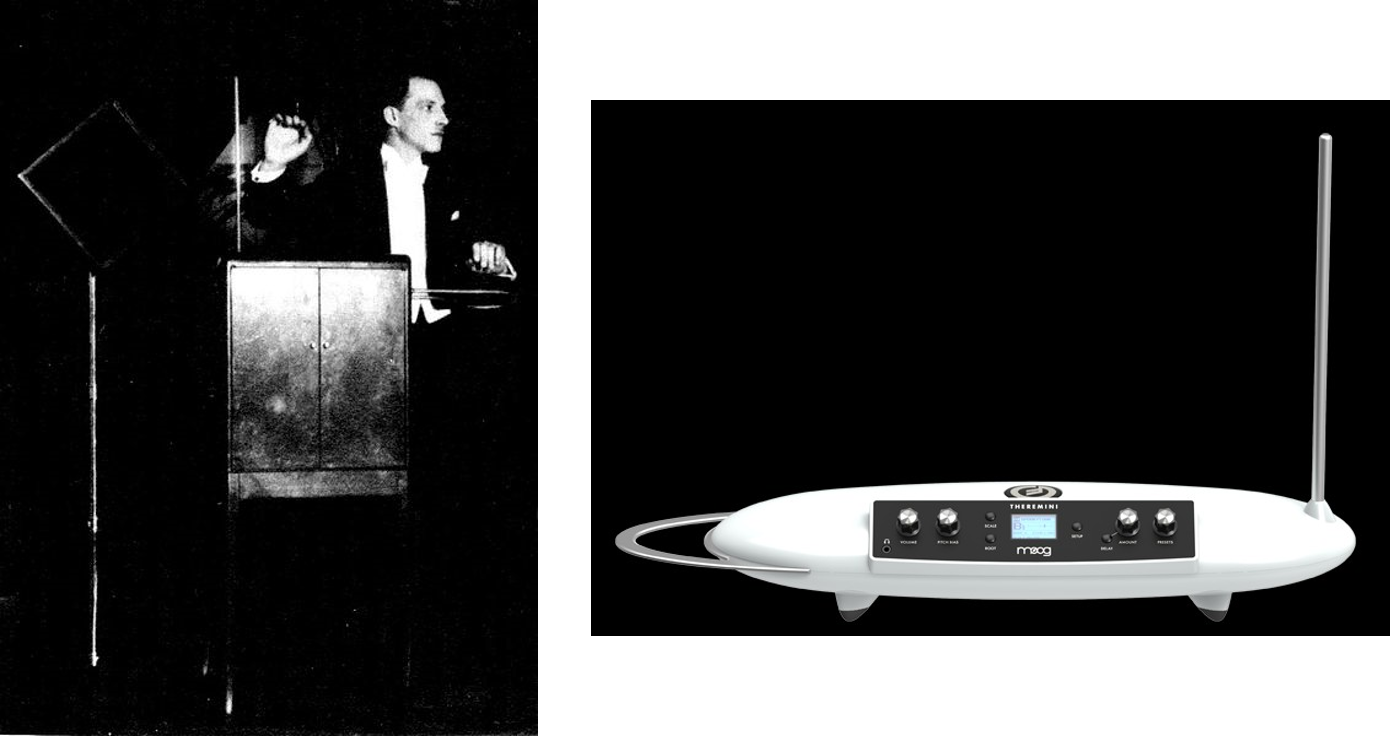
\includegraphics[width=0.9\textwidth]{images/theremins}
\captionof{figure}{\emph{Left:} Leon Theremin playing his epnoymous electronic musical instrument \cite{Glinsky2000}. \emph{Right:} The Theremini by Moog Music Inc., released in 2014 \cite{moog2014}}
\label{fig:theremins}
\end{minipage}
In the last decades of the 19th and the beginning of the 20th century a considerable number of inventors and scientists performed research on the application of electric systems, sparking innovations such as electric lighting, electric motors, telegraphy, and radio communication. Lev Sergeyevich Termen or Léon Theremin in the American naming was a Russian inventor most famous for designing the eponymous theremin. This early electronic musical instrument could be played without touch. One hand is controlling the pitch and the other the volume by changing the distance to an antenna. Initially designed as a motion detector, this device is transferring the influence of the human body on an oscillating electric field to an audible sound \cite{Glinsky2000}. Léon Theremin can be seen playing the instrument in Figure \ref{fig:theremins} on the left. This instrument is still in production to this day, with the electronic music instrument company Moog releasing a new variety that simplifies the sound production by fitting the distance to a sound on a specific musical scale \cite{moog2014}. The instrument is shown in Figure \ref{fig:theremins} on the right.

Electric field imaging was a research focus at the MIT in the 1990s. A research group in the Media Lab division including Joseph A. Paradiso, Thomas G. Zimmerman, Joshua R. Smith designed various sensing devices and evaluated various applications in in the domains of human computer interaction, smart appliances and reactive systems. They drew inspiration from biological precedents - various species of fish, such as Gymnotoidei can sense their surroundings using electric fields \cite{Smith1999a}. The changing currents created by objects with a different dielectric constant from water can be registered and thus used to avoid obstacles, even if no light source is available. Accordingly, the group named some of their prototypes after this biological precedent, including the LazyFish and School of Fish \cite{Smith1999a}. The research group created various different applications in the domains of human computer interaction, smart appliances and reactive systems.

\begin{minipage}{\linewidth}
\centering
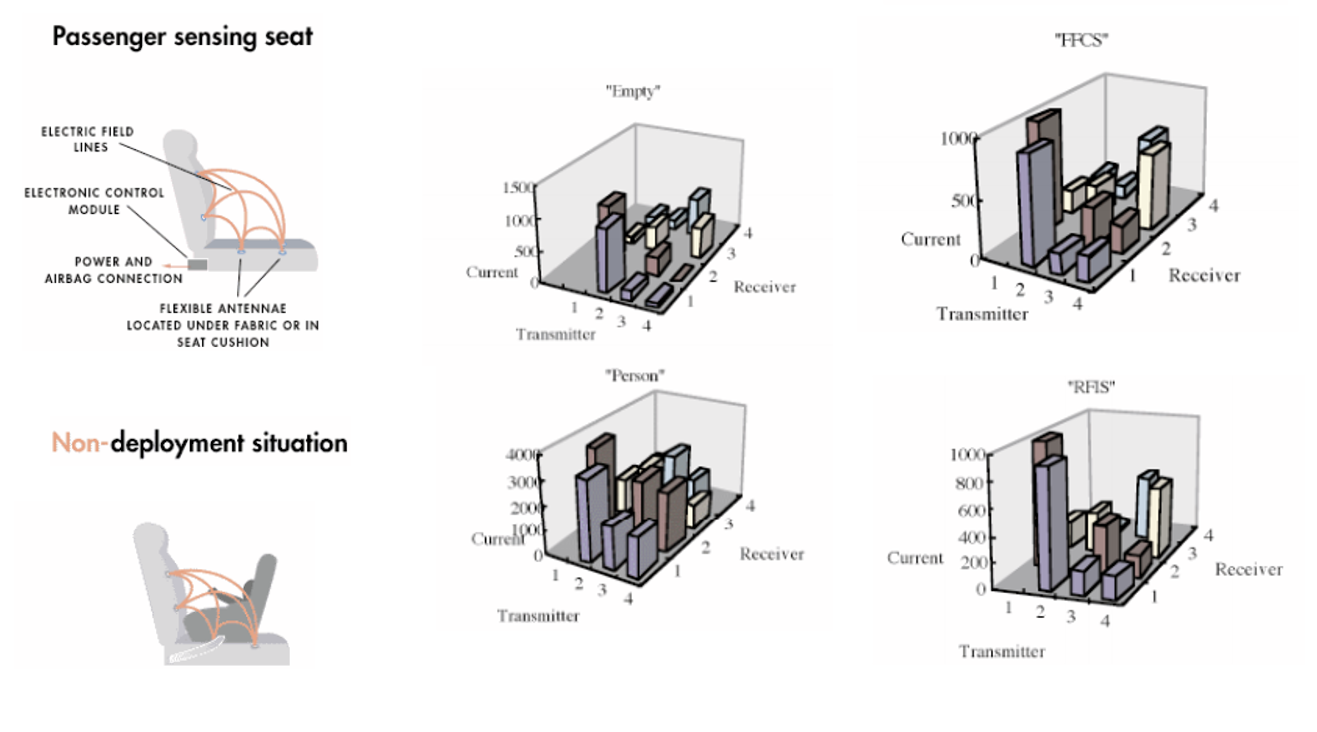
\includegraphics[width=0.9\textwidth]{images/nec_passenger_seat}
\captionof{figure}{\emph{Left:} Concept view of passenger seat set to deploy or not deploy airbag. \emph{Center:} Sensor readings for empty seat and adult person. \emph{Right:} Sensor readings for front-facing child seat (FFCS) and rear-facing child seat (RFCS). \cite{Smith1999a}}
\label{fig:nec_passenger_seat}
\end{minipage}

In collaboration with NEC a smart passenger seat was created that incorporated capacitive sensors operating in shunt mode to detect if an infant seat is currently present on the passenger seat of car \cite{Smith1999a}. The underlying challenge is that an airbag deployment should be prevented in such cases to prevent potential injuries to the infant. The seat is able to distinguish four different states, “No passenger”, “adult passenger”, “front-facing infant seat” and “rear-facing infant seat”. It uses four sending and four receiving electrodes and classifies the situation according to the current readings - the concept and readings of the sensors in the different situations are shown in Figure \ref{fig:nec_passenger_seat}.

\begin{minipage}{\linewidth}
\centering
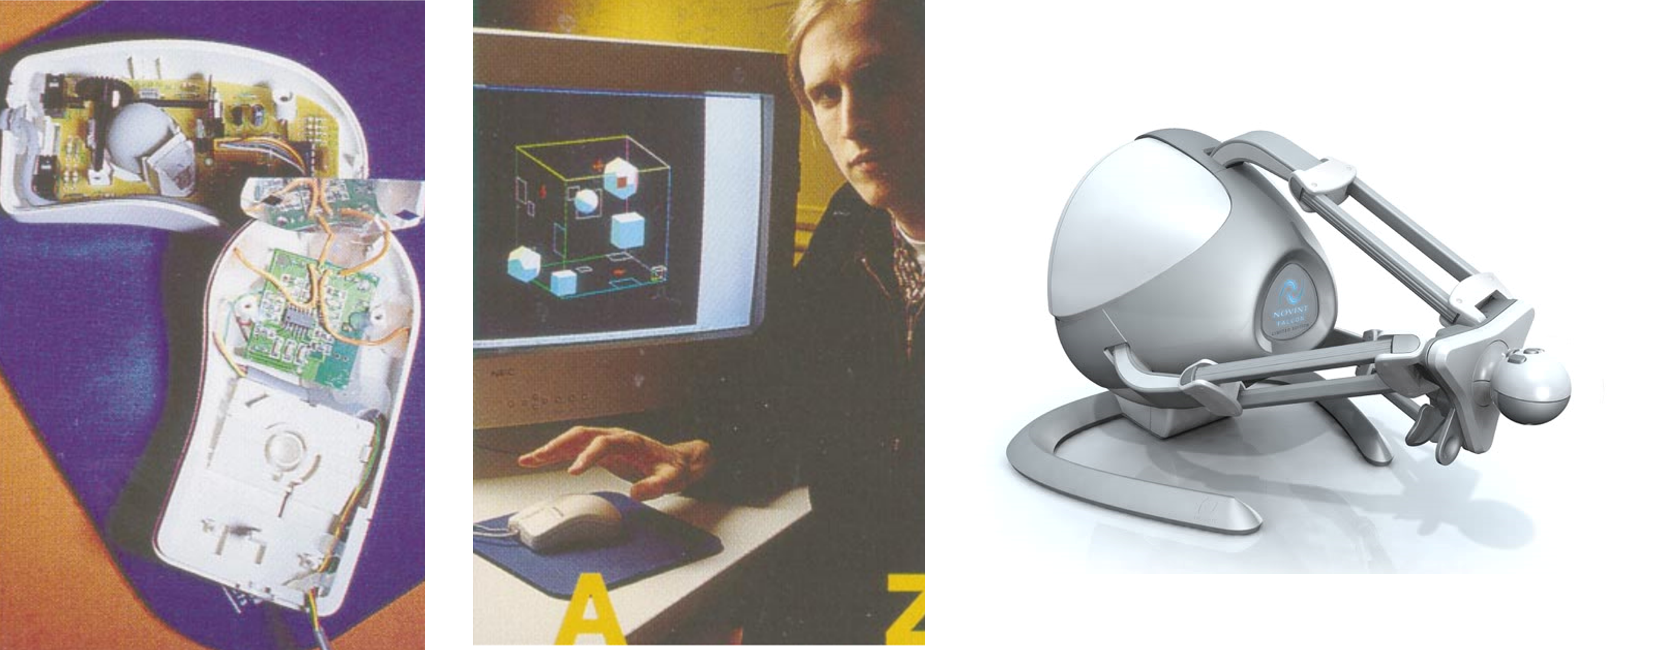
\includegraphics[width=0.9\textwidth]{images/lazmouse}
\captionof{figure}{\emph{Left:} LaZmouse innards \emph{Center:} Joshua R. Smith using LaZmouse \cite{Smith1999a} \emph{Right:} Novint Falcon 3D input device \cite{novint2014}}
\label{fig:lazmouse}
\end{minipage}

Another prototype is the LaZmouse that extends a regular mouse with shunt mode capacitive sensors, having one transmitting and two receiving electrodes, to measure the proximity between the heel of the hand from the mouse surface, thus allowing the fingers to remain in the common position and the mouse to be moved around \cite{Smith1999a}. Effectively this creates an input device with three degrees-of-freedom, enabling to perform interactions with a mouse that would usually require a more specialized 3D input device, such as the Novint Falcon that tracks the movement of the moved interaction sphere in three dimensions \cite{novint2014}. Figure \ref{fig:lazmouse} shows on the left, the electronics inside the mouse, the inventor using the device and a graphical representation, and on the right the Novint Falcon.

In another work Paradiso et al. presented numerous applications for capacitive proximity sensors, including smart furniture devices \cite{ Zimmerman1995}. They propose a smart table, comprised of a single transmitter electrode and two receivers that is able to track the position of a hand in two dimensions, a chosen dimension on the table and height. It may be used as gesture input device or to augment video desk applications. They also installed the system in a room, whereas the floor is a single electrode and there are four receivers located on the walls. This allows to infer the location of a person, based on relative signal strength. An additional system in this work is the smart chair, using a single transmitter in the seat and four receivers in the armrests and headrest. It allows to navigate through various audio channels based on head and arm movements \cite{ schmandt1995audiostreamer}.

\begin{minipage}{\linewidth}
\centering
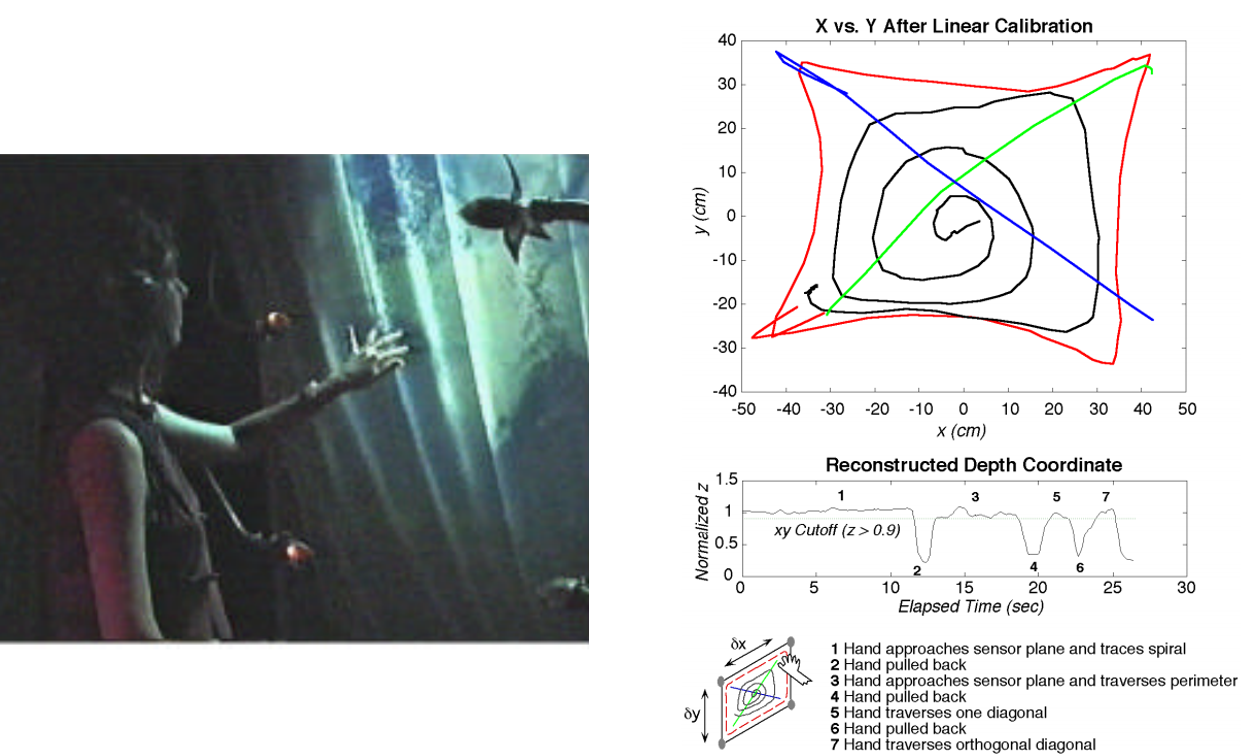
\includegraphics[width=0.8\textwidth]{images/related_gesture_wall}
\captionof{figure}{\emph{Left:} Person interacting with the gesture wall  \emph{Right:} Air drawing results, depth estimation results and associated movements on bottom. \cite{smith1998electric}}
\label{fig:related_gesture_wall}
\end{minipage}

A final prototype of this group I would like to present is the Gesture Wall, a large interactive multimedia wall, designed for public appearances \cite{smith1998electric}. A plate on the floor in front of the screen is acting as transmitter and four receiving electrodes that protruded from the edges of the projection area, as shown in Figure \ref{fig:related_gesture_wall}. It supports interactive experiences, such as drawing in the air, controlling different audio streams and an interactive video clip.

\begin{minipage}{\linewidth}
\centering
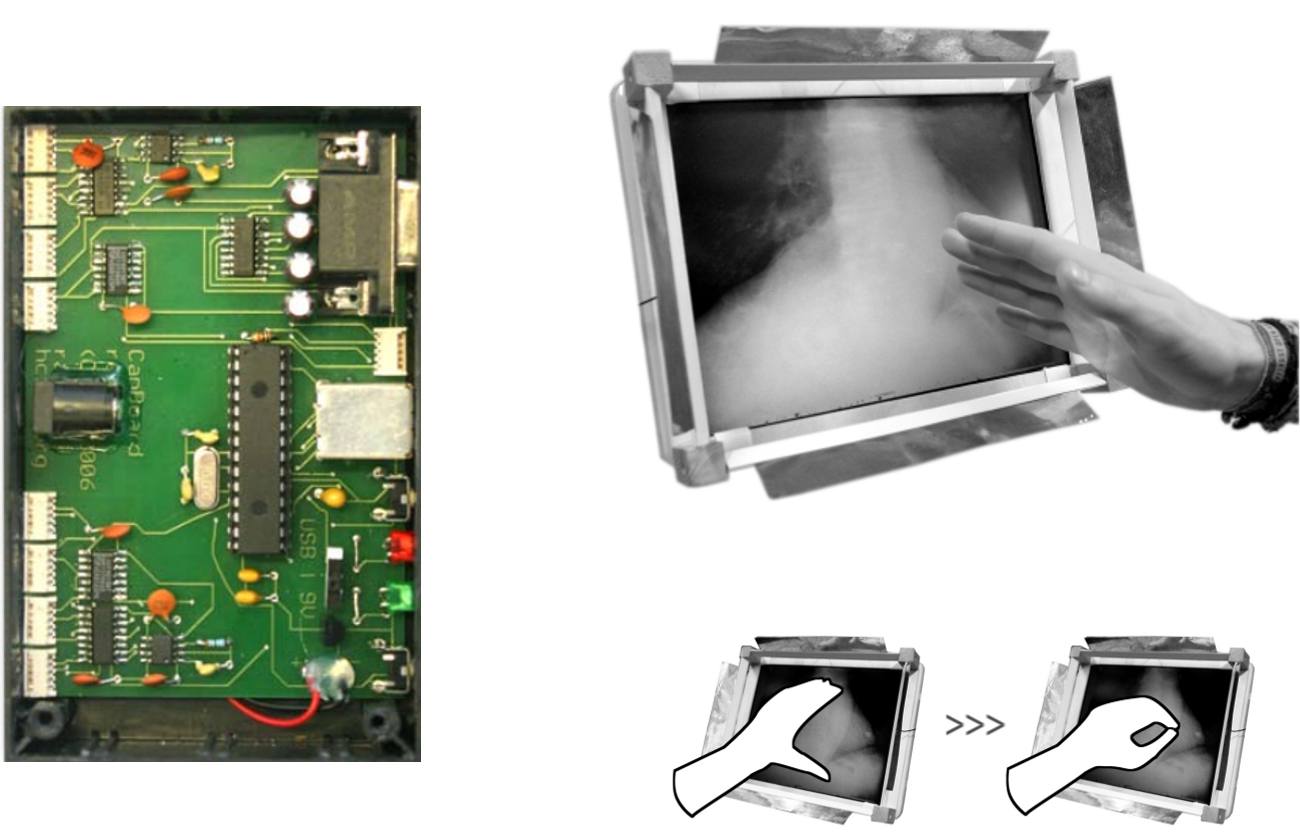
\includegraphics[width=0.9\textwidth]{images/related_ctk_thracker}
\captionof{figure}{\emph{Left:} Prototype of CapToolKit  \cite{Wimmer2007a} \emph{Right:} Thracker prototype and visualized grasping gestures. \cite{Wimmer2006}}
\label{fig:related_ctk_thracker}
\end{minipage}

Another group that was active in capacitive proximity sensing was located at the University of Munich. Raphael Wimmer and colleagues revisited capacitive sensors in the scope of human-computer interaction. They created CapToolKit, a capacitive sensing rapid prototyping toolkit that allows interfacing eight capacitive proximity sensors and enables a quick design and testing of new applications  \cite{Wimmer2007a}. They also created Thracker - a display augmented with four capacitive proximity sensors that allows to detect the position of the hand in front of the screen and supports performed pick-and-drop gestures \cite{Wimmer2006}. Both devices are shown in Figure\ref{fig:related_ctk_thracker}.

\begin{minipage}{\linewidth}
\centering
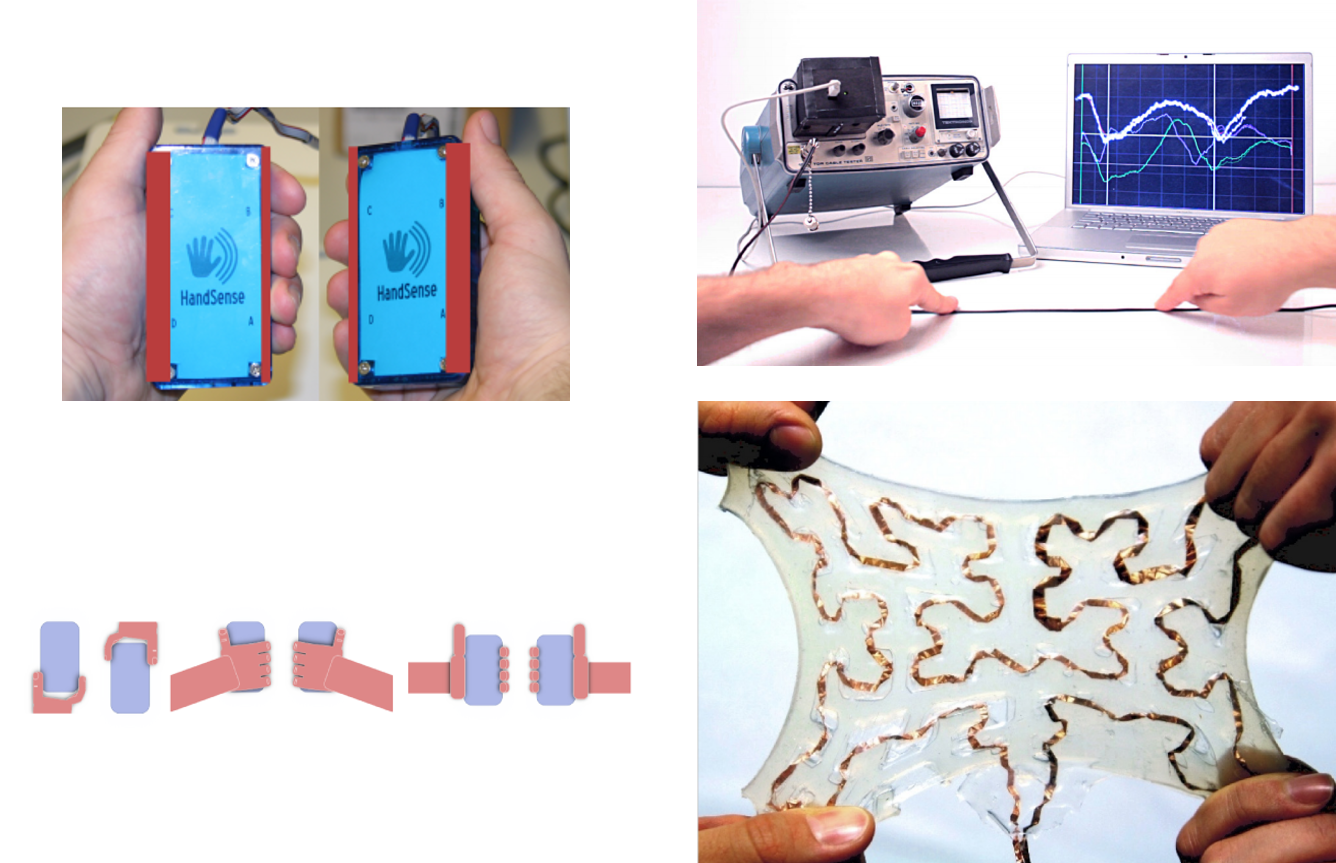
\includegraphics[width=0.8\textwidth]{images/related_handsense_tdr}
\captionof{figure}{\emph{Left:} Prototype of HandSense and supported grasping types \cite{wimmer2009handsense}. \emph{Right:} Setup of time domain reflectometry sensing and example of stretchable material \cite{wimmer2011modular}.}
\label{fig:related_handsense_tdr}
\end{minipage}

In other works they also presented capacitive sensing to allow discriminating the ways an interaction device is held, including distinguishing left and right hand or proximity to a body part \cite{ wimmer2009handsense}. This enables graphical interfaces to be adapted, based on user-handedness, grasping style and spatial cues that can be acquired from this device in collaboration with other sensors. Supported grasping styles and a prototype are shown in Figure \ref{fig:related_handsense_tdr}, on the left.

A final work of this group was concerned with exploring the potential of time domain reflectometry for human-computer interaction \cite{wimmer2011modular}. This technique is sending a short electrical pulse into an electric conductor and measures the time until the signal returns. Originally intended for finding defects in long cables, such as transatlantic phone lines, high-sampling rates enable to also detect the presence of grounding objects close to much shorter conductors. Wimmer and Baudisch use an image analysis on the screen of an older reflectometer to enable applications, such as location tracking, touch detection and stretchable materials. The setup and an example of stretchable materials are shown in Figure \ref{fig:related_handsense_tdr}, on the right.

\begin{minipage}{\linewidth}
\centering
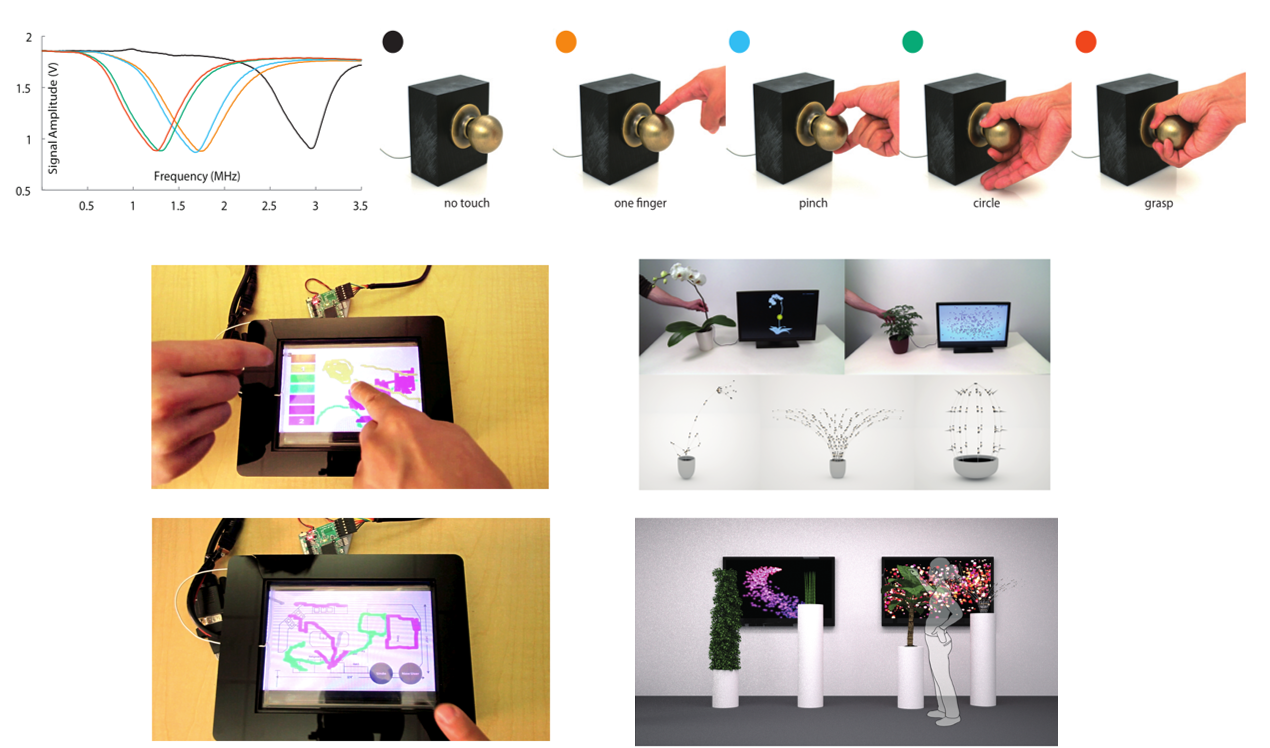
\includegraphics[width=0.8\textwidth]{images/rel_cap_disney}
\captionof{figure}{\emph{Top:} Capacitive profiles of different gestures on a door knob \cite{Sato2012}. \emph{Bottom Left:} User identification using capacitive fingerprinting \cite{harrison2012capacitive}. \emph{Bottom Right:} Botanicus Interacticus prototype and interaction concept \cite{poupyrev2012botanicus}} 
\label{fig:rel_cap_disney}
\end{minipage}

Another research group that has been recently active with capacitive sensing systems is centered around Ivan Poupyrev. They presented Touché, proposing a novel sensing technology called swept-frequency capacitive sensing \cite{Sato2012}. Instead of relying on a single excitation frequency like typical capacitive sensors this measurement system is sweeping a larger range of frequencies, thus allowing to get more data points from a single electrode. Many systems react differently to changing frequencies, including the human body and its complex structure of bone, muscle, fat and other tissues. The result is a capacitive profile comprised of values at different frequencies, as shown in Figure \ref{fig:rel_cap_disney} on the top. Using these profiles it is possible to distinguish numerous events based on the application, e.g. the different ways in which a mobile device can be held. Other applications proposed in this work were sensing of body postures on a table, on-body gestures using wrist-worn sensors, interaction with a body of water and grasping a door knob using different gestures. Building on this work Harrison et al. proposed a system using this technology to identify the users of a touch screen with a capacitive fingerprint \cite{harrison2012capacitive}. This allows to distinguish the touches of different users, thus enabling a variety of applications on collaboratively used touch screen devices, such as gaming and multiuser drawing tools, as shown in Figure \ref{fig:rel_cap_disney} on the bottom left. An interesting suggestion are personalized undo stacks that allow a more seamless collaboration. A final system is the Botanicus Interacticus, that uses the same technology to realize interactive installations using plants  \cite{poupyrev2012botanicus}. It is possible to distinguish the location a certain plant is touched and associate it to different input events. In this first system it was used in an interactive art installation, that is shown in Figure \ref{fig:rel_cap_disney} on the bottom right.

\begin{minipage}{\linewidth}
\centering
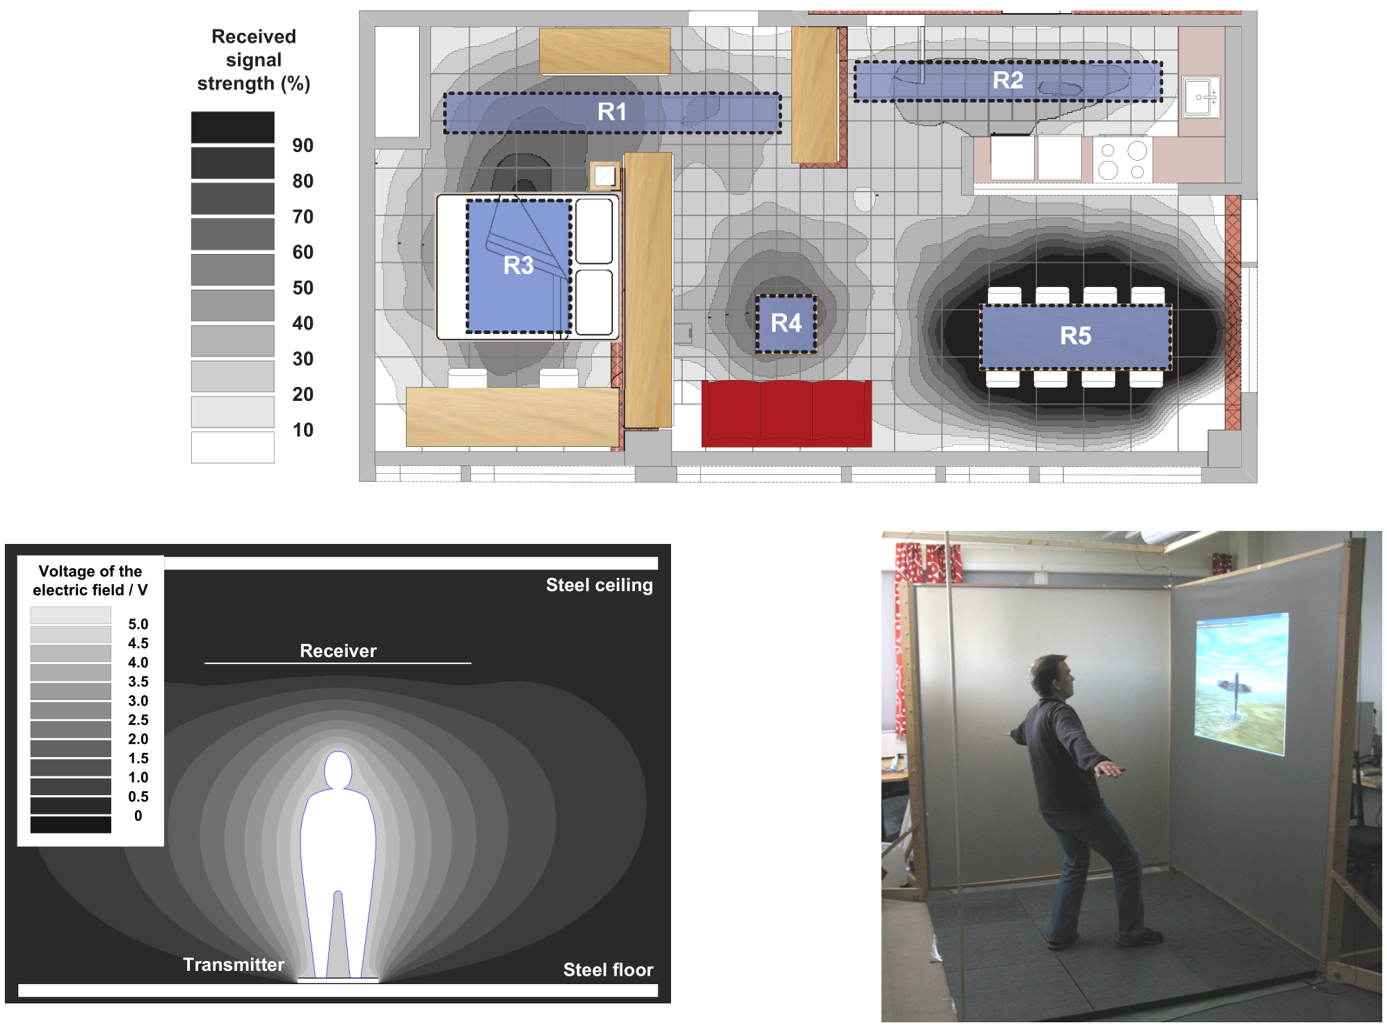
\includegraphics[width=0.8\textwidth]{images/rel_cap_tampere}
\captionof{figure}{\emph{Top:} Capacitive profiles of different gestures on a door knob \cite{Sato2012}. \emph{Bottom Left:} User identification using capacitive fingerprinting \cite{harrison2012capacitive}. \emph{Bottom Right:} Botanicus Interacticus prototype and interaction concept \cite{poupyrev2012botanicus}} 
\label{fig:rel_cap_tampere}
\end{minipage}

A final group working with capacitive proximity sensing that I would like to present is located at the Tampere University of Technology. Valtonen et al. have been working on a capacitive proximity sensing system tracking the position of users in a room \cite{Valtonen2009a,valtonen2012capacitive}. A transmitting electrode is placed under the floor and several receiver electrodes are hidden in the walls or other objects of the room. The system therefor is using the presented transmit mode, coupling the users present in the environment to an electrode in the floor and measuring the effect on the receiver electrodes. A downside of this system is the required proximity to a wall electrode, making application in larger rooms impossible. Accordingly, an addition was presented that hides the receiving electrodes in different items of furniture to provide a more reliable localization in living environments \cite{valtonen2012capacitive}. The placement of the receiver electrodes (R) and the received signal strength in the environment are shown in Figure \ref{fig:rel_cap_tampere} on the top. An extension of this principle is using a similar electrode configuration to  determine height and posture of a person between a transmitter electrode on the bottom and a receiver electrode on the ceiling \cite{valtonen2011unobtrusive}. A simulation of the electric field voltages created in this setup is shown in Figure \ref{fig:rel_cap_tampere} on the bottom left. The taller a person, the higher the resulting signal. Accordingly, a sitting or lying person will have a much smaller effect and can be classified. A similar setup was also used to identify different gestures performed in an interaction area, as shown in Figure \ref{fig:rel_cap_tampere} on the bottom right \cite{valtonen2010human}. Using a single transmitter and four wire receivers in the corners it is possible to track different body postures and control some example applications.


